% Verify-Agents @ NeurIPS 2026 (Sydney) workshop poster: 61 cm wide x 85 cm high, portrait.
% Built on the unofficial QRS template (neurips26-poster.sty, workshop option). The .sty is
% unchanged; colours, header and footer are overridden locally below (Stanford palette).
% Previous versions: poster_backup_2026-11-11.tex, poster_backup_2026-11-15b.tex (+ .pdf).
%
% Sources of truth: camera-ready paper (../neuripsworkshoppaper.tex) and saved artifacts.
% Each number's source is given in a % comment beside it. Provenance audit: crit_artifact_audit.md.
% Figures: make_poster_figures.py (asserts plotted values reproduce the saved analyses).
%
% Venue facts (checked 11 Nov 2026): poster ID 172969 (neurips.cc/virtual/2026/loc/sydney/poster/172969);
% workshop Sat 12 Dec 2026, Hall 5; poster sessions 11:00-12:00 and 14:45-15:45 AEDT;
% workshop posters 61 cm W x 85 cm H portrait, not larger (neurips.cc/Conferences/2026/PosterInstructions).
\documentclass{article}
\usepackage[workshop]{neurips26-poster}
\usepackage{booktabs}
\usepackage{sansmath}
\usetikzlibrary{positioning,arrows.meta,calc,fit,backgrounds}

% ------------------------------------------------------------------ Stanford palette
\definecolor{cardinal}{HTML}{8C1515}
\definecolor{deepcardinal}{HTML}{820000}
\definecolor{charcoal}{HTML}{2E2D29}
\definecolor{lightneutral}{HTML}{F7F7F7}
\definecolor{midgray}{HTML}{767674}
\definecolor{palered}{HTML}{F9EEEE}
% Template colour names -> Stanford roles
\definecolor{npink}{HTML}{8C1515}     % section headings
\definecolor{npaccent}{HTML}{8C1515}  % divider rules, key-result accent
\definecolor{nppaper}{HTML}{FFFFFF}   % page
\definecolor{npsoft}{HTML}{F9EEEE}    % key-result fill
\pagecolor{white}

\title{Do Reasoning-Quality Metrics Predict Better Decisions?\\[0.2em]
  {\fontsize{40}{48}\selectfont\mdseries Verifying multi-agent debate against external market outcomes}}
\author{Juli Huang, Alanood Alrassan, Deveen Harischandra, Theodore Wu, Veljko Skarich, Matthew Hayes}
\affiliation{Stanford University}
\paperurl{https://neurips.cc/virtual/2026/loc/sydney/poster/172969}
\posterid{172969}
\newcommand{\codeurl}{https://github.com/TheClassicTechno/cs372research}
\session{Who Verifies the Agents? Toward Reliable Agent Development\\NeurIPS 2026 Workshop, Sydney \textbullet\ Sat 12 Dec, Hall 5}
\contact{julih@stanford.edu}

\newcommand{\pp}{\,pp}
\newcommand{\postersmall}{\fontsize{22}{28}\selectfont}
\newcommand{\postertiny}{\fontsize{20}{25}\selectfont}
\newcommand{\posterref}{\fontsize{17}{21}\selectfont}
\newcommand{\rhobar}{\ensuremath{\bar{\rho}}}
\newcommand{\illus}[1]{{\postertiny\color{midgray}#1}}

\makeatletter
% Header: deep Cardinal band, white title/authors, light-neutral affiliation.
\renewcommand{\makeheader}{%
  \begin{tcolorbox}[enhanced, colback=deepcardinal, colframe=deepcardinal, arc=0pt, boxrule=0pt,
      left=\np@gap, right=\np@gap, top=0.6\np@gap, bottom=0.6\np@gap, frame hidden]
    \color{white}\raggedright
    {\fontsize{58}{66}\selectfont\bfseries\np@title\par}\vspace{0.35em}
    {\np@authorsize\np@authors\quad{\color{lightneutral}\itshape\textbullet\ \np@affiliations}\par}
  \end{tcolorbox}\vspace{0.45\np@gap}}
% Footer: venue + contact | references | QR to the poster page.
\setlength{\np@qr}{3.6cm}
\renewenvironment{block}[1]{%
  \begin{tcolorbox}[enhanced, breakable=false, colback=white, colframe=white, arc=0pt, boxrule=0pt,
      left=0pt, right=0pt, top=0pt, bottom=0.2\np@gap, spartan]
  {\fontsize{34}{40}\selectfont\bfseries\color{cardinal}#1\par}\vspace{-0.2em}
  {\color{cardinal}\rule{4cm}{1.6mm}}\par\vspace{-0.1em}}{\end{tcolorbox}}
\renewcommand{\makefooter}{%
  \vfill
  {\color{cardinal}\rule{\linewidth}{2mm}}\par\vspace{0.15\np@gap}
  \np@footsize\color{charcoal}
  \begin{minipage}[c]{21cm}\raggedright
    \textbf{\np@session}\par\vspace{0.1em}
    Poster \np@posterid\quad\np@contact\par
    {\posterref QR: poster page on neurips.cc. Code: \texttt{\codeurl}}\par
  \end{minipage}\hfill
  \begin{minipage}[c]{\dimexpr\linewidth-21cm-\np@qr-2\np@gap\relax}\raggedright\posterref
    \textbf{References}\par\vspace{0.15em}
    [1]~E.\,Y.~Chang. Prompting large language models with the Socratic method. arXiv:2303.08769, 2023.\par
    [2]~E.\,Y.~Chang, L.~Geng. RAudit: A blind auditing protocol for large language model reasoning. arXiv:2601.23133, 2026.\par
    [3]~V.~DeMiguel, L.~Garlappi, R.~Uppal. Optimal versus naive diversification: How inefficient is the 1/N portfolio strategy? \emph{Rev.\ Financ.\ Stud.}~22(5), 2009.\par
  \end{minipage}\hfill
  \begin{minipage}[c]{\np@qr}\raggedleft\qrcode[height=\np@qr]{\np@paperurl}\end{minipage}}
\makeatother

\tikzset{
  pbox/.style={draw=charcoal, line width=0.8mm, fill=lightneutral, rounded corners=2.5mm,
    align=center, inner sep=3mm, font=\postersmall},
  hbox/.style={pbox, draw=cardinal, fill=white},
  arr/.style={line width=1.1mm, -{Stealth[length=6mm,width=6mm]}, draw=charcoal},
}

\begin{document}
\sansmath
\color{charcoal}
\makeheader
\postertext\setlength{\parskip}{0.3em}

%% ================================================================ full width: finding, problem, real run
\begin{minipage}[t]{0.5\linewidth}\vspace{0pt}
\begin{block}{Can agents argue better without deciding better?}
  AI financial agents analyze historical market information, allocate a simulated \$100{,}000
  portfolio, and sometimes debate. We score their reasoning with a rubric, \textbf{CRIT}, then
  compare those scores with independently measured \textbf{next-quarter market outcomes}.
\end{block}
\end{minipage}\hfill
\begin{minipage}[t]{0.47\linewidth}\vspace{0pt}
\begin{keyresult}
  \raggedright
  % rq1_clustered_stats.json: pooled:sharpe r=0.0735, ci95 [-0.130, 0.254]
  {\fontsize{32}{39}\selectfont\bfseries Higher reasoning scores showed little association
  with better realized financial outcomes in our tested scenarios.\par}\vspace{0.25em}
  {\postertext Across 210 runs, CRIT vs.\ next-quarter Sharpe: $r{=}{+}0.07$,
  95\%~CI~$[-0.13, +0.25]$.\par}
\end{keyresult}
\end{minipage}
\par\vspace{-0.4cm}

\begin{block}{One real run: the start of 2022}
  % CS372_210_debate_runs/logging/runs/vskarich_ablation_7/run_2026-03-11_16-12-13_003
  % (A7 baseline, scenario_2022Q1). Verified 2026-11-15:
  %   shared_context/memo.txt: as-of 2021-12-31; CPI YoY 7.17%; 2Y +45bps QoQ; WTI $75.33
  %   rounds/round_001/proposals/{macro,technical}/portfolio.json (top weights shown)
  %   rounds/round_001/{critiques,revisions}/ present (one critique-revise round)
  %   final/final_portfolio.json: MSFT .12, CVX .10, NVDA .10, _CASH_ .06
  %   final/pid_crit_all_rounds.json: rho_bar 0.87
  %   _dashboard/financial_metrics.json: return -0.195%, SPY -5.16%, Sharpe 0.054, max DD 10.05%
  \begin{tikzpicture}[every node/.style={pbox, text width=8.7cm, minimum height=3.3cm}]
    \node[anchor=west] (memo) at (0,0) {\textbf{1. Market memo}, 31 Dec 2021\\
      CPI 7.2\%, 2-yr yield $+$45\,bp, oil \$75; filings and news on 21 stocks};
    \node[anchor=west, minimum height=2.5cm] (mac) at (11.4,1.45) {\textbf{2. Macro agent}\\ CVX 10, XOM 10\% \ldots};
    \node[anchor=west, minimum height=2.5cm] (tec) at (11.4,-1.45) {\textbf{2. Technical agent}\\ NVDA 18, AMD 12\% \ldots};
    \node[anchor=west, fill=palered, draw=cardinal] (rev) at (22.8,0) {\textbf{3. Debate}\\ each critiques the other's proposal, then revises};
    \node[anchor=west] (fin) at (34.2,0) {\textbf{4. Final portfolio}\\ (LLM judge): MSFT 12, CVX 10, NVDA 10, \ldots, cash 6\%};
    \node[anchor=west, hbox, fill=palered, text width=8.8cm] (out) at (45.6,0) {\textbf{5. Outcome, 2022 Q1}\\
      return $-0.2\%$ (S\&P 500 ETF $-5.2\%$); Sharpe 0.05; max drawdown 10\%};
    \node[hbox, anchor=north, text width=23cm, minimum height=1.6cm] (crit) at ($(rev.south)+(0,-1.0)$)
      {\textbf{CRIT} grades the arguments: $\bar\rho = 0.87$ (0--1). It never sees 2022 prices
       and is told not to judge outcomes.};
    \node[draw=none, fill=none, anchor=north west, text width=14.5cm, align=left, minimum height=0pt]
      at ($(crit.north east)+(1.0,0.1)$)
      {All values: one saved run (A7 baseline). Red border: realized \emph{after} the decision.};
    \draw[arr] (memo.east) -- (mac.west);
    \draw[arr] (memo.east) -- (tec.west);
    \draw[arr] (mac.east) -- (rev.west);
    \draw[arr] (tec.east) -- (rev.west);
    \draw[arr] (rev.east) -- (fin.west);
    \draw[arr, draw=cardinal] (fin.east) -- (out.west);
    \draw[arr] (rev.south) -- (crit.north);
  \end{tikzpicture}
\end{block}

%% ================================================================ two columns
\vspace{-0.4cm}
\begin{columns}{2}
%% ---------------------------------------------------------------- column 1: how we test
\begin{block}{How we test: ensemble vs.\ debate}
  % configs: vote_*_no_macro*.yaml (propose_only, judge_type average);
  % debate_1_round_*.yaml and A7/A8/A10 (critique + revise, judge_type llm)
  \begin{tikzpicture}[node distance=0.35cm and 0.9cm, every node/.style={font=\postersmall}]
    \node[anchor=west, text width=4.4cm] (h0) at (0,1.65) {\textbf{Baseline}};
    \node[pbox, right=0.2cm of h0] (s1) {one agent decides alone};
    \node[anchor=west, text width=4.4cm] (h1) at (0,0) {\textbf{Ensemble}};
    \node[pbox, right=0.2cm of h1] (e1) {separate proposals};
    \node[pbox, right=of e1] (e2) {average weights};
    \draw[arr] (e1) -- (e2);
    \node[anchor=west, text width=4.4cm] (h2) at (0,-1.65) {\textbf{Debate}};
    \node[pbox, right=0.2cm of h2] (d1) {proposals};
    \node[pbox, fill=palered, draw=cardinal, right=of d1] (d2) {critique, revise};
    \node[pbox, right=of d2] (d3) {LLM judge picks};
    \draw[arr] (d1) -- (d2); \draw[arr] (d2) -- (d3);
  \end{tikzpicture}

\end{block}

\begin{block}{CRIT: grading the argument}
  % CRIT prompt in each run: rounds/round_001/CRIT/<agent>/prompt.txt; paper Sec. 2
  An LLM grader (\texttt{gpt-5}) [1, 2] scores each agent's case 0--1:
  \par\vspace{0.1em}
  {\postersmall\setlength{\tabcolsep}{0.3em}
  \begin{tabular}{@{}ll@{}}
    \textbf{P1 Logic} & does the allocation follow from the argument? \\
    \textbf{P2 Evidence} & are claims backed by cited memo data? \\
    \textbf{P3 Alternatives} & are critiques and rival views addressed? \\
    \textbf{P4 Causal} & is each causal claim backed by a mechanism? \\
  \end{tabular}\par}
  \vspace{0.1em}
  {\postersmall Agent score $\rho_i$ = mean of 4 pillars; run score $\bar\rho$ = mean over agents.
  The grader is not the judge that picks the portfolio.\par}
\end{block}


\begin{block}{Three prompt styles}
  % multi_agent/prompts: roles/*_slim.txt; system_contract/system_causal_contract.txt;
  % system_contract/enriched_reasoning_debate_protocol.txt (+ enumeration phase templates)
  {\postersmall\setlength{\tabcolsep}{0.3em}
  \begin{tabular}{@{}l p{0.74\linewidth}@{}}
    \textbf{Basic} & role description; cite memo evidence \\
    \textbf{Causal} & $+$ mechanisms, confounders, reverse causation \\
    \textbf{Enriched} & $+$ numbered claims, assumptions, falsifiers \\
  \end{tabular}\par}
  \vspace{0.1em}
  % paper Sec. 4 / tab:crit_gains; author records, logs not recovered (paper App., crit_artifact_audit.md)
  {\postersmall Previously reported, separate runs: enriched prompts raised CRIT 0.72$\to$0.84.
  These prompts ask for what CRIT rewards, so scores can rise by compliance.\par}
\end{block}

\begin{block}{RQ1: Does higher CRIT go with better outcomes?}
  % analysis/rq1/per_run_results.csv (CS372_210_debate_runs) -> rq1_clustered_stats.json; paper Table 1
  % within:sharpe r=-0.0218, ci95 [-0.164, 0.115]
  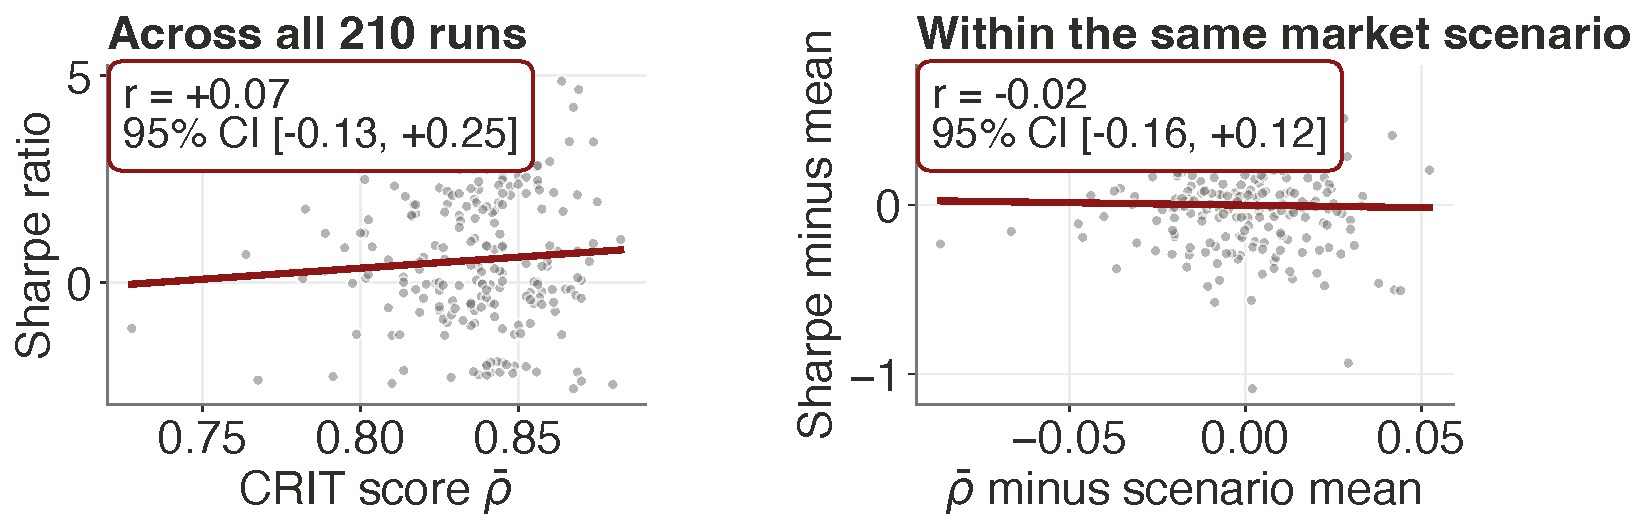
\includegraphics[width=\linewidth]{fig_crit_vs_sharpe.pdf}
  \par
  {\postersmall 210 runs (35 scenarios $\times$ 6 conditions). Pearson $r$: linear association (0 = none).
  CIs resample whole scenarios (same-scenario runs are dependent).\par}
  \textbf{No clear linear link detected;} the pooled CI still allows a modest positive one.
\end{block}

%% ---------------------------------------------------------------- column 2: what we found
\nextcolumn


\begin{block}{RQ2: Do prompts and debate help the portfolio?}
  % analysis/verify_paper_tables.csv (tab:prompts, paired_vs=A); bands: results/seed_variance
  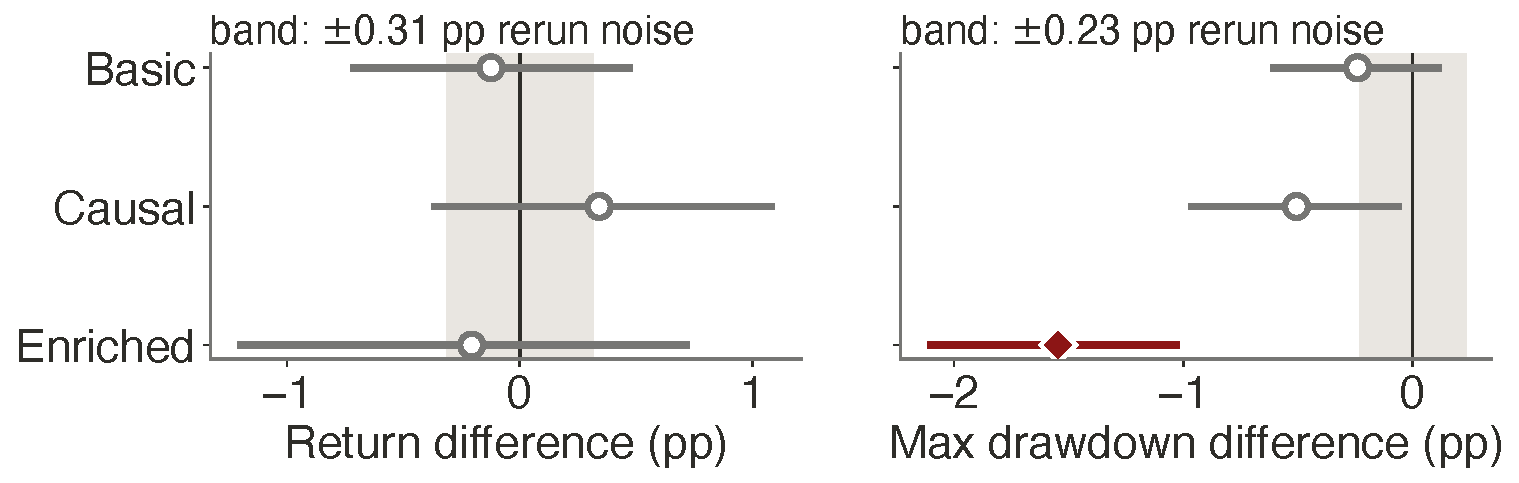
\includegraphics[width=\linewidth]{fig_effect_vs_noise.pdf}
  \par
  {\postersmall 3-agent ensemble minus single agent, 35 paired scenarios; dot = mean, line = 95\%
  CI (pp = percentage points). Gray band = rerun noise per metric, a scale reference, not a
  significance test. \textbf{Max drawdown}: largest peak-to-trough fall.\par}
  \begin{itemize}
    % tab:prompts col D: max DD -1.545 [-2.11, -1.02], p<0.001; cash ~8% -> 17%
    \item \textbf{Enriched: shallower drawdown} ($-1.5$\pp), partly from holding more cash
      (8\%\,$\to$\,17\%). No return change exceeds the noise.
    % tab:debate_rca col B vs A
    \item \textbf{Debate vs.\ ensemble:} drawdown $-0.45$\pp\ ($p{=}0.018$); return and
      Sharpe not better.
    % tab:debate_vs_ew, pooled 455 runs
    \item Debate beat an equal-weight portfolio [3] in only \textbf{33\%} of 455 runs.
  \end{itemize}
\end{block}

\begin{block}{RQ3: Can targeted retries fix debate?}
  % vskarich_ablations/ablation_{7,8,10}/debate_configs; eval/interventions/rules.py;
  % analysis/rq1/per_run_results.csv (paired t, 35 scenarios); tab:paired-ttests
  {\postersmall If a problem is detected, agents redo their revision. \textbf{JSD}: how different
  agents' portfolios are; $\mathrm{JS}_{\text{rev}}/\mathrm{JS}_{\text{prop}}$ = share of
  disagreement left after revising. \textbf{Sharpe}: annualized risk-adjusted return.\par}
  \vspace{0.4em}
  {\setlength{\tabcolsep}{0.7em}
  \begin{tabular}{@{}l@{\hspace{1.2em}}ccc@{}}
    \toprule
    \textbf{Retry when\ldots} & \textbf{Agents} & \textbf{Change in Sharpe} & \textbf{$p$-value} \\
    \midrule
    A7: $\mathrm{JS}_{\text{rev}}/\mathrm{JS}_{\text{prop}}<0.8$ & 2 & \textbf{+0.14} & \textbf{0.028} \\
    A8: same rule & 3 & $+0.04$ & 0.53 \\
    A10: CRIT $P_4<0.75$ & 2 & $-0.09$ & 0.22 \\ % ablation_10/debate_configs/causal_intervention_th075.yaml
    \bottomrule
  \end{tabular}\par}\vspace{0.4em}
  % revision limit = prompt instruction (runner.py ~L1249), followed in 38/42 A7 retries
  % (analysis/rq1/intervention_audit.json); Bonferroni x3: 0.028 -> 0.084
  {\postersmall A7 showed a positive Sharpe difference, but $p$ is uncorrected for 3 tests
  (Bonferroni 0.08). Its retry prompt also limited revisions (${\le}2$ stocks, ${\le}5$ points
  each), so no single mechanism is isolated. A10 raised the causal score, not Sharpe.\par}
\end{block}
\end{columns}

%% ================================================================ full width: lessons + scope
\vspace{0.4cm}
\begin{minipage}[t]{0.13\linewidth}\raggedright
  {\fontsize{34}{40}\selectfont\bfseries\color{cardinal}Three\\lessons\par}
\end{minipage}\hfill
\begin{minipage}[t]{0.275\linewidth}\raggedright
  \textbf{1. Convincing argument $\neq$ better decision.}\par
  {\postersmall CRIT was weakly associated with realized outcomes here.\par}
\end{minipage}\hfill
\begin{minipage}[t]{0.275\linewidth}\raggedright
  \textbf{2. Design changed risk more than return.}\par
  {\postersmall Some setups cut drawdown; steady excess return was not shown.\par}
\end{minipage}\hfill
\begin{minipage}[t]{0.275\linewidth}\raggedright
  \textbf{3. Debate needs meaningful baselines.}\par
  {\postersmall Compare with one agent and with averaged independent agents.\par}
\end{minipage}
\par\vspace{0.6em}
% paper Sec. 5 (Limitations); provenance: paper Appendix (recovered artifacts), crit_artifact_audit.md
{\postersmall\textbf{Scope.} 35 scenarios (2021\,Q4--25\,Q3) of 3--35 stocks each, \texttt{gpt-5-mini} agents; no
trading costs; possible pre-training recall. Some prompt-evaluation records are unavailable (see paper).\par}

\makefooter
\end{document}
